\documentclass[12pt]{article}

% TEMPLATE DEFAULT PACKAGES
\usepackage{amssymb,amsmath,amsfonts,eurosym,geometry,ulem,graphicx,color,setspace,sectsty,comment,natbib,pdflscape,array,adjustbox}

% ADDED PACKAGES FOR THIS MANUSCRIPT
\usepackage{palatino,newtxmath,multirow,titlesec,threeparttable,tabu,booktabs,titlesec,threeparttable,mathtools,bm,bbm,subcaption,pdflscape,tcolorbox,mathrsfs}
% endfloat,

\usepackage{afterpage}
\usepackage[hyphens]{url}
\usepackage[margin=1cm]{caption}

\usepackage[draft]{hyperref}
\newcommand{\tim}{$\,\times\,$}
% FIGURES & TABLES CAPTION STYLING
\captionsetup[figure]{labelfont={bf},name={Figure},labelsep=period}
\captionsetup[table]{labelfont={bf},name={Table},labelsep=period}

% SECTION TITLE SETTINGS
\titlelabel{\thetitle.\enskip}
\titleformat*{\section}{\large\bfseries}
\titleformat*{\subsection}{\normalsize\bfseries}

% COLUMN TYPES
\newcolumntype{L}[1]{>{\raggedright\let\newline\\\arraybackslash\hspace{0pt}}m{#1}}
\newcolumntype{C}{>{\centering\arraybackslash}p{5.2em}}
\newcolumntype{D}{>{\centering\arraybackslash}p{5em}}
\newcolumntype{R}[1]{>{\raggedleft\let\newline\\\arraybackslash\hspace{0pt}}m{#1}}


% MARGINS AND SPACING
\normalem
\geometry{left=1.1in,right=1.1in,top=1.0in,bottom=1.0in}
\setlength{\parskip}{2.5pt}

% SPECIAL CELL 
\newcommand{\specialcell}[2][c]{%
	\begin{tabular}[#1]{@{}l@{}}#2\end{tabular}}

% NO INDENT ON FOOTNOTES
\usepackage[hang,flushmargin]{footmisc}

\begin{document}



\vspace{0mm}
\begin{table}[h!]
\centering
\caption{Housing Project Areas Description}\label{table:projectdescriptives}
\vspace{0mm}
\begin{tabular}{l*{1}{cccccc}}
\toprule
  & \multicolumn{2}{c}{\textbf{All}}& \multicolumn{2}{c}{\textbf{Greenfield}}  & \multicolumn{2}{c}{\textbf{In-Situ}}   \\
  &Const. & Unconst. &Const. & Unconst.   & Const. & Unconst. \\
\midrule
 Number of Projects  & 172  & 145  & 43  & 20  & 27  & 29  \\ 
 Area (km2)  & 1.17  & 1.16  & 1.72  & 2.42  & 1.50  & 0.88  \\ 
 Median Construction Yr.  & 2006  & 2006  & 2006  & 2005  & 2004  & 2006  \\ 
 Delivered Houses  & 374  & 11  & 568  & 24  & 702  & 20  \\ 
 House Price in 1 km (R$^\dagger$)  & 188,441  & 218,635  & 194,214  & 186,841  & 179,596  & 208,570  \\ 
 Distance to CBD$^\ddagger$ (km)  & 32.5  & 27.7  & 40.5  & 39.9  & 32.6  & 30.6  \\ 

\bottomrule
\multicolumn{7}{l}{\scriptsize Const. refers to constructed projects and unconst. refers to unconstructed projects.}\\[-.5em]
\multicolumn{7}{l}{\scriptsize $^*$Calculated from {\it expected} completion dates using Gauteng National Treasury budget reports.}\\[-.5em]
\multicolumn{7}{l}{\scriptsize $^\dagger$ The USD averaged to about 7.70 Rands during the 2001-2011 period.}\\[-.5em]
\multicolumn{7}{l}{\scriptsize $^\ddagger$Measured as the average minimum distance with respect to Johannesburg and Pretoria CBDs. } \\[-.5em]
%\multicolumn{7}{l}{\scriptsize City includes projects whose centroids are within 30.4 km of their nearest CBD.} \\[-.5em]
%\multicolumn{7}{l}{\scriptsize Suburb includes projects whose centroids are further than 30.4 km from their nearest CBD.}
\end{tabular}
\end{table} 



\begin{figure*}
        \centering
   %     \caption[ Pre-Period Housing Densities in Constructed and Unconstructed Projects Areas ]
  %      {\small Pre-Period Densities} 
        %\vspace{2mm}
        \begin{subfigure}[b]{0.48\textwidth}
                    \caption[Network2]%
            {{\footnotesize \textbf{All Projects} pre-period formal raw data}}    
            \label{fig:prefor}
            \centering
            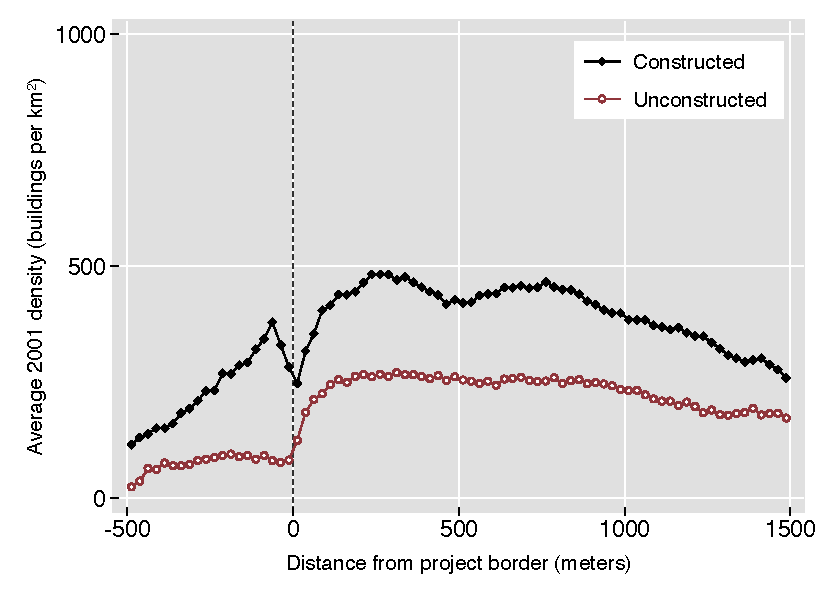
\includegraphics[width=\textwidth,trim={0.3cm .3cm 0.1cm 0cm}, clip=true]{figures/bblu_for_pre_means_4_spk.pdf}

        \end{subfigure}
        \hfill
        \begin{subfigure}[b]{0.48\textwidth}  
                    \caption[]%
            {{\footnotesize \textbf{All Projects} pre-period informal  raw data}}      
            \label{fig:preinf}
            \centering 
            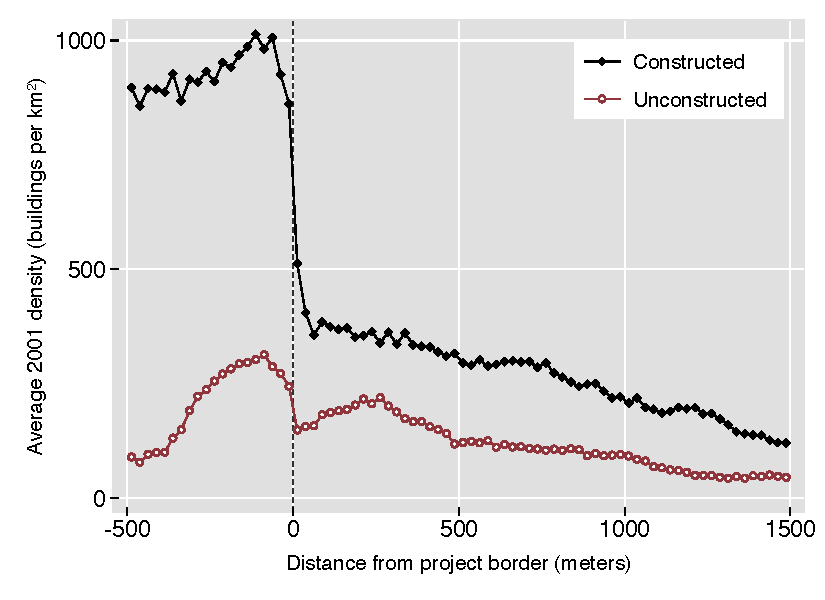
\includegraphics[width=\textwidth,trim={0.3cm .3cm 0.1cm 0cm}, clip=true]{figures/bblu_inf_pre_means_4_spk.pdf}

        \end{subfigure}
        \begin{subfigure}[b]{0.48\textwidth}
                    \caption[Network2]%
            {{\footnotesize \textbf{Greenfield} pre-period formal  raw data}}    
            \label{fig:prefor}
            \centering
            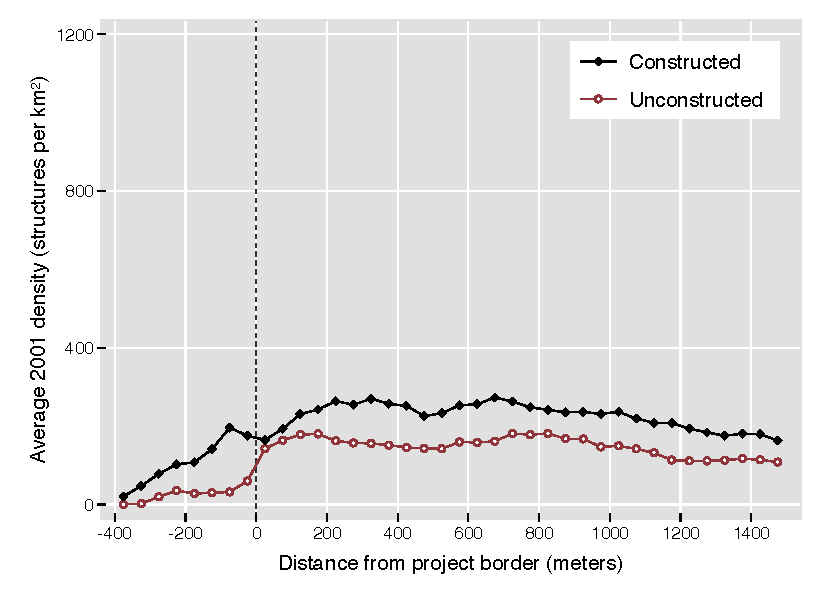
\includegraphics[width=\textwidth,trim={0.3cm .3cm 0.1cm 0cm}, clip=true]{figures/bblu_for_pre_means_4_1_spk.pdf}

        \end{subfigure}
        \hfill
        \begin{subfigure}[b]{0.48\textwidth}  
                    \caption[]%
            {{\footnotesize \textbf{Greenfield} pre-period informal  raw data}}     
            \label{fig:preinf}
            \centering 
            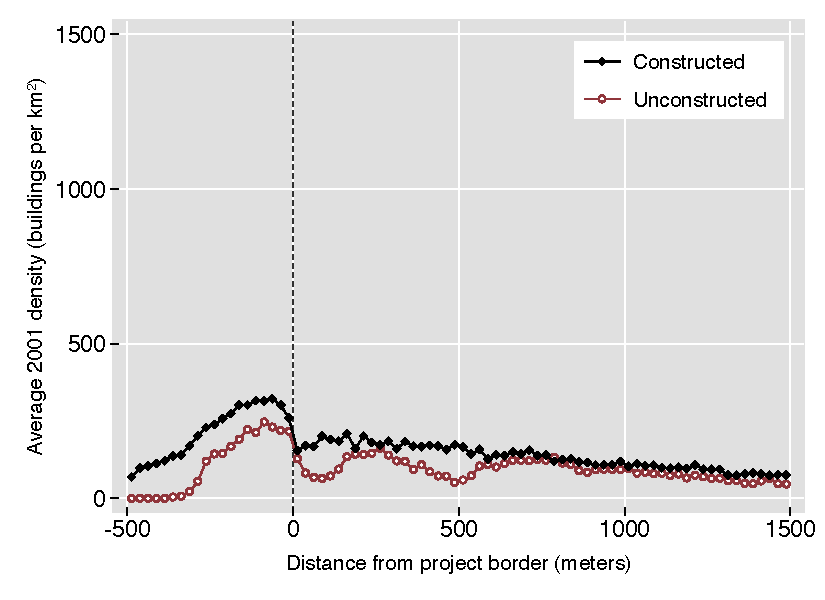
\includegraphics[width=\textwidth,trim={0.3cm .3cm 0.1cm 0cm}, clip=true]{figures/bblu_inf_pre_means_4_1_spk.pdf}

        \end{subfigure}
        \begin{subfigure}[b]{0.48\textwidth}
                    \caption[Network2]%
            {{\footnotesize \textbf{In-Situ} pre-period formal  raw data}}   
            \label{fig:prefor}
            \centering
            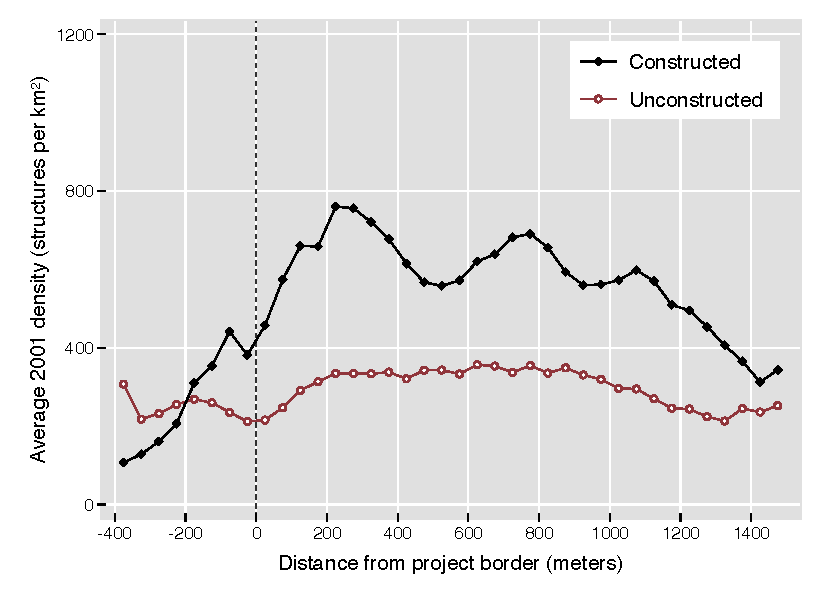
\includegraphics[width=\textwidth,trim={0.3cm .3cm 0.1cm 0cm}, clip=true]{figures/bblu_for_pre_means_4_2_spk.pdf}

        \end{subfigure}
        \hfill
        \begin{subfigure}[b]{0.48\textwidth}  
                    \caption[]%
            {{\footnotesize \textbf{In-Situ} pre-period informal  raw data}}     
            \label{fig:preinf}
            \centering 
            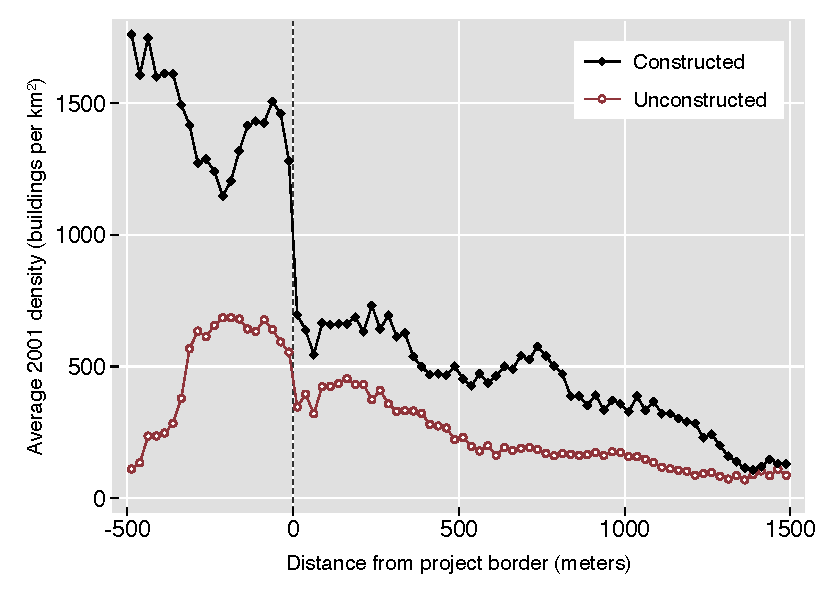
\includegraphics[width=\textwidth,trim={0.3cm .3cm 0.1cm 0cm}, clip=true]{figures/bblu_inf_pre_means_4_2_spk.pdf}

        \end{subfigure}
        \begin{subfigure}[b]{0.48\textwidth}
                    \caption[Network2]%
            {{\footnotesize \textbf{Other} pre-period formal  raw data}}   
            \label{fig:prefor}
            \centering
            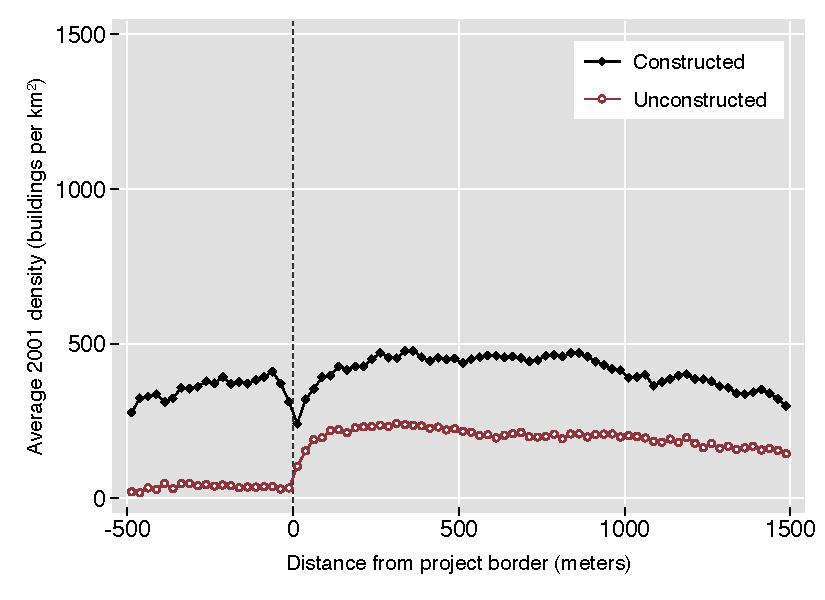
\includegraphics[width=\textwidth,trim={0.3cm .3cm 0.1cm 0cm}, clip=true]{figures/bblu_for_pre_means_4_3_spk.pdf}

        \end{subfigure}
        \hfill
        \begin{subfigure}[b]{0.48\textwidth}  
                    \caption[]%
            {{\footnotesize \textbf{Other} pre-period informal  raw data}}      
            \label{fig:preinf}
            \centering 
            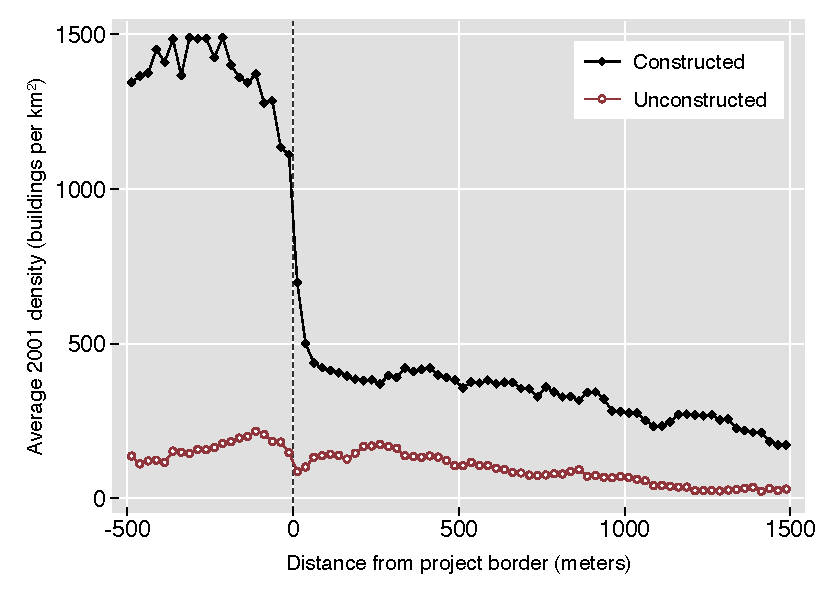
\includegraphics[width=\textwidth,trim={0.3cm .3cm 0.1cm 0cm}, clip=true]{figures/bblu_inf_pre_means_4_3_spk.pdf}

        \end{subfigure}
\end{figure*}








\begin{figure*}
        \centering
   %     \caption[ Pre-Period Housing Densities in Constructed and Unconstructed Projects Areas ]
  %      {\small Pre-Period Densities} 
        %\vspace{2mm}
        \begin{subfigure}[b]{0.48\textwidth}
            \caption[Network2]%
            {{\footnotesize \textbf{All Projects} changes formal raw data}}    
            \label{fig:prefor}
            \centering
            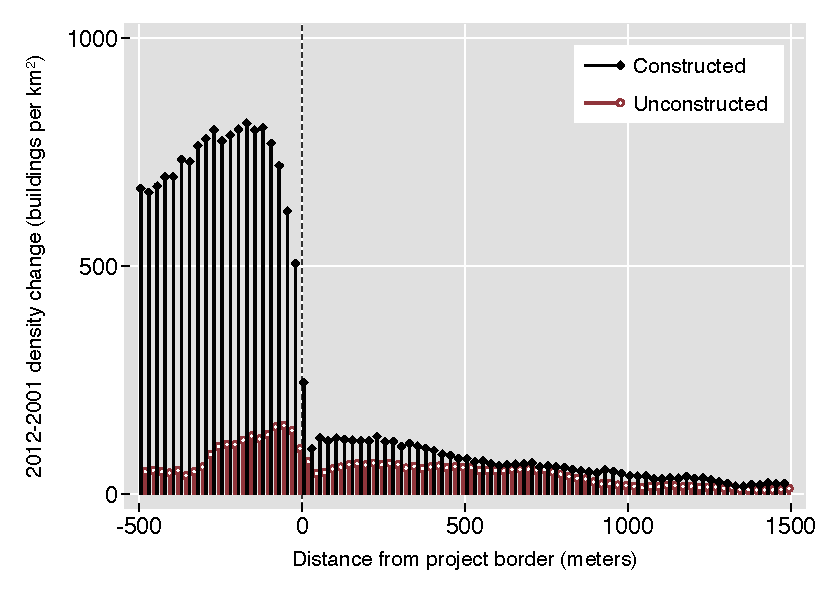
\includegraphics[width=\textwidth,trim={0.3cm .3cm 0.1cm 0cm}, clip=true]{figures/bblu_for_rawchanges_4_spk.pdf}

        \end{subfigure}
        \hfill
        \begin{subfigure}[b]{0.48\textwidth}  
                    \caption[]%
            {{\footnotesize \textbf{All Projects} changes informal  raw data}}      
            \label{fig:preinf}
            \centering 
            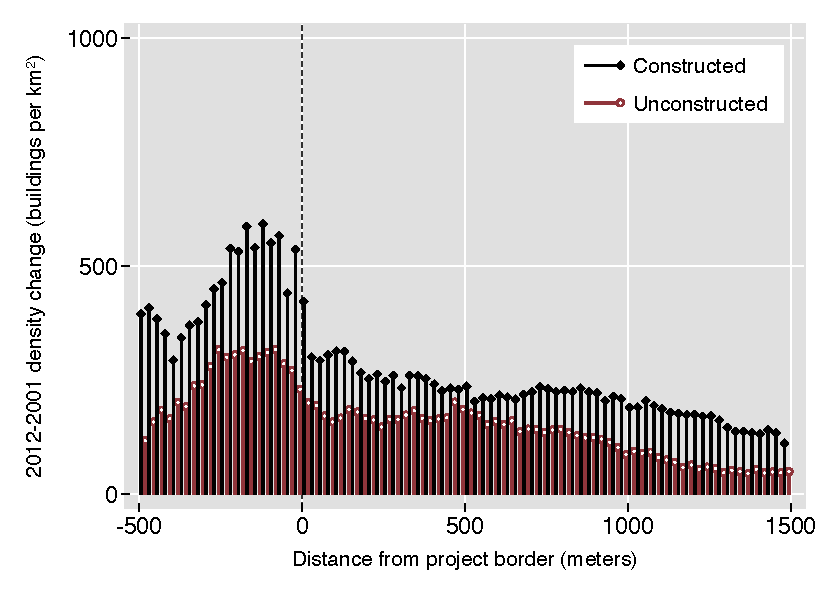
\includegraphics[width=\textwidth,trim={0.3cm .3cm 0.1cm 0cm}, clip=true]{figures/bblu_inf_rawchanges_4_spk.pdf}

        \end{subfigure}
        \begin{subfigure}[b]{0.48\textwidth}
                    \caption[Network2]%
            {{\footnotesize \textbf{Greenfield} changes formal  raw data}}    
            \label{fig:prefor}
            \centering
            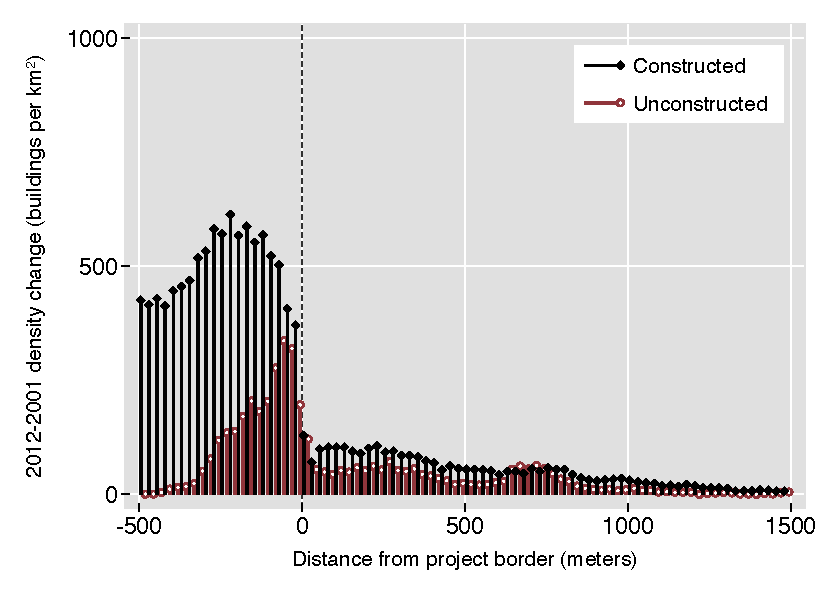
\includegraphics[width=\textwidth,trim={0.3cm .3cm 0.1cm 0cm}, clip=true]{figures/bblu_for_rawchanges_4_1_spk.pdf}

        \end{subfigure}
        \hfill
        \begin{subfigure}[b]{0.48\textwidth}  
                    \caption[]%
            {{\footnotesize \textbf{Greenfield} changes informal raw data }}     
            \label{fig:preinf}
            \centering 
            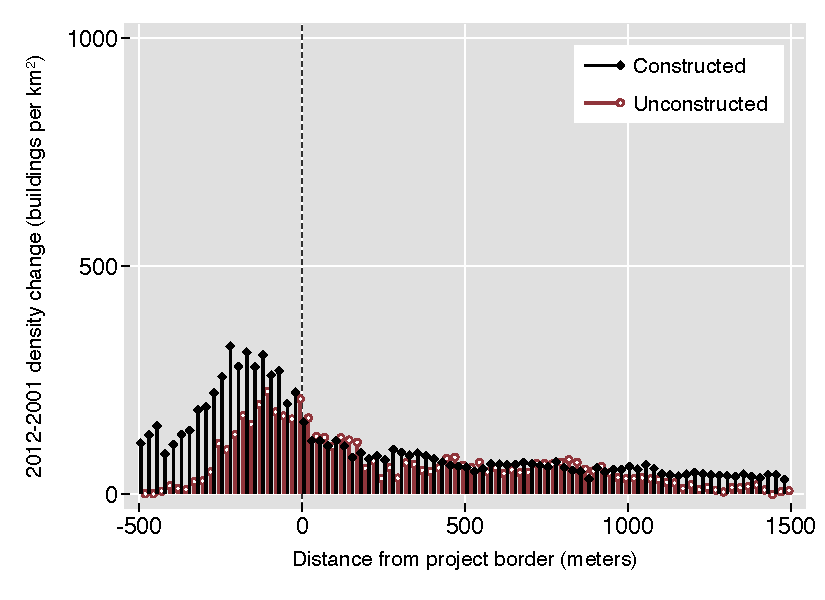
\includegraphics[width=\textwidth,trim={0.3cm .3cm 0.1cm 0cm}, clip=true]{figures/bblu_inf_rawchanges_4_1_spk.pdf}

        \end{subfigure}
        \begin{subfigure}[b]{0.48\textwidth}
                    \caption[Network2]%
            {{\footnotesize \textbf{In-Situ} changes formal raw data }}   
            \label{fig:prefor}
            \centering
            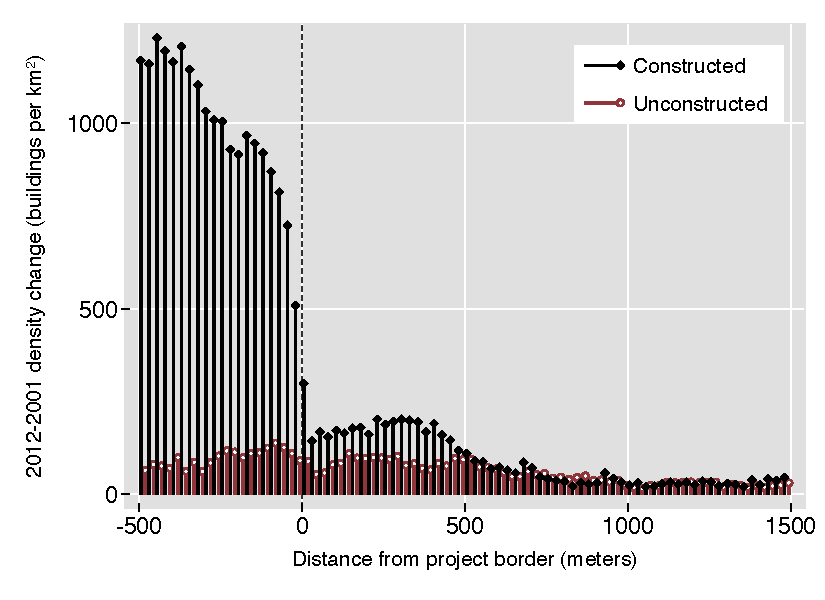
\includegraphics[width=\textwidth,trim={0.3cm .3cm 0.1cm 0cm}, clip=true]{figures/bblu_for_rawchanges_4_2_spk.pdf}

        \end{subfigure}
        \hfill
        \begin{subfigure}[b]{0.48\textwidth}  
                    \caption[]%
            {{\footnotesize \textbf{In-Situ} changes informal raw data }}     
            \label{fig:preinf}
            \centering 
            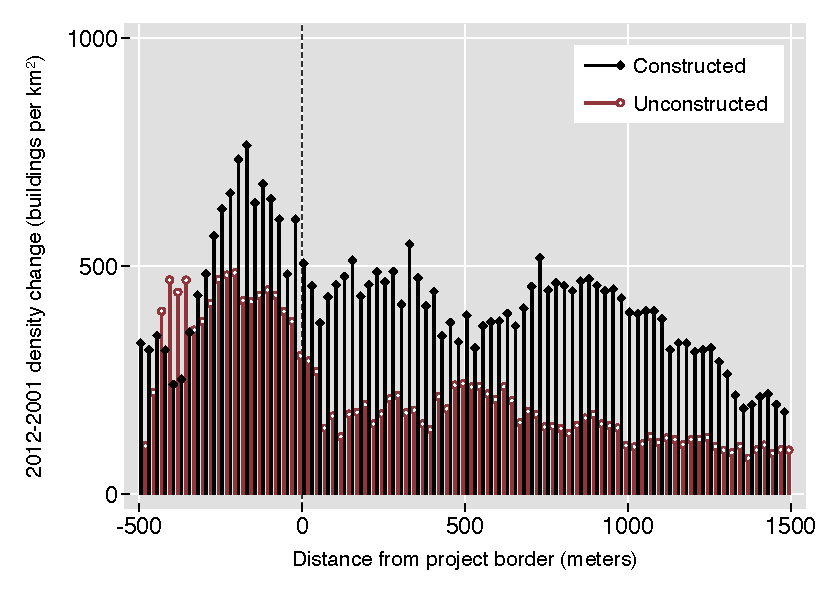
\includegraphics[width=\textwidth,trim={0.3cm .3cm 0.1cm 0cm}, clip=true]{figures/bblu_inf_rawchanges_4_2_spk.pdf}

        \end{subfigure}
        \begin{subfigure}[b]{0.48\textwidth}
                    \caption[Network2]%
            {{\footnotesize \textbf{Other} changes formal raw data}}   
            \label{fig:prefor}
            \centering
            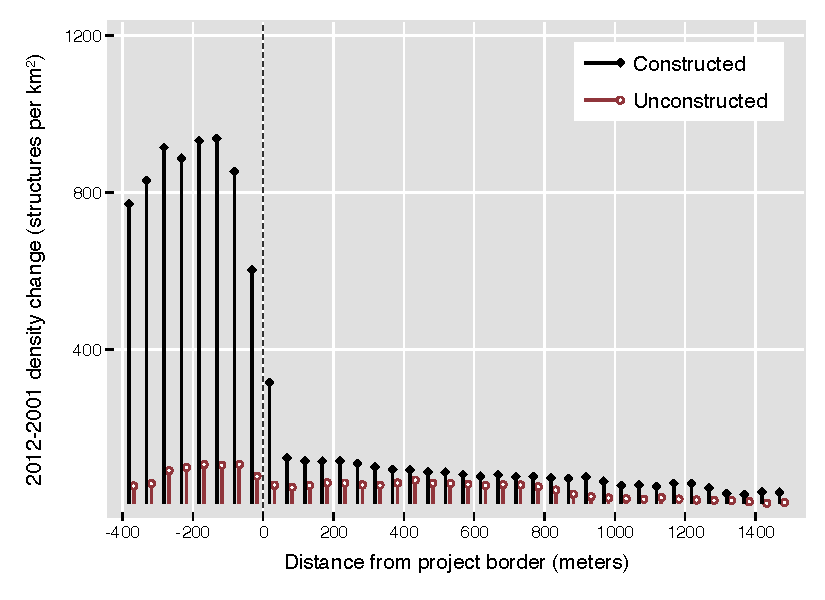
\includegraphics[width=\textwidth,trim={0.3cm .3cm 0.1cm 0cm}, clip=true]{figures/bblu_for_rawchanges_4_3_spk.pdf}

        \end{subfigure}
        \hfill
        \begin{subfigure}[b]{0.48\textwidth} 
                    \caption[]%
            {{\footnotesize \textbf{Other} changes informal  raw data}}      
            \label{fig:preinf} 
            \centering 
            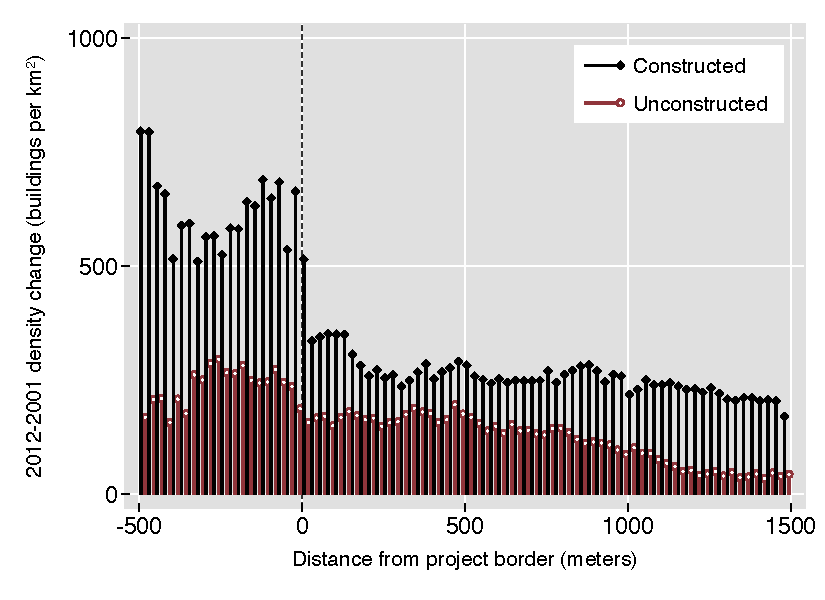
\includegraphics[width=\textwidth,trim={0.3cm .3cm 0.1cm 0cm}, clip=true]{figures/bblu_inf_rawchanges_4_3_spk.pdf}

        \end{subfigure}
\end{figure*}







\begin{table}
\caption{Building Density}
\begin{tabular}{lDDDDD}
\toprule
 & \small (1) & \small (2)  & \small (3) & \small (4) & \small (5) \\
 & Total & Formal  & Informal & Informal Bkyd. & Informal Non-Bkyd. \\ \midrule
\textbf{All Projects} \\inside project      &     794.726\textsuperscript{a}&     621.182\textsuperscript{a}&     173.544\textsuperscript{c}&     567.515\textsuperscript{a}&    -393.971\textsuperscript{a}\\
                    &   (140.541)                   &    (73.454)                   &    (96.156)                   &    (99.385)                   &    (80.913)                   \\[0.5em]
0-300m outside project &      80.724\textsuperscript{c}&      58.137\textsuperscript{b}&      22.587                   &      63.421\textsuperscript{c}&     -40.833                   \\
                    &    (47.916)                   &    (23.098)                   &    (41.037)                   &    (34.741)                   &    (29.003)                   \\[0.5em]
300-600m outside project &     -21.967                   &      13.999                   &     -35.966                   &      -4.244                   &     -31.722\textsuperscript{c}\\
                    &    (33.027)                   &    (13.783)                   &    (28.677)                   &    (25.441)                   &    (17.169)                   \\[0.5em]
R$^2$               &       0.072                   &       0.050                   &       0.061                   &       0.049                   &       0.045                   \\

\midrule
\textbf{Greenfield} \\   inside project      &     486.025\textsuperscript{b}&     350.687\textsuperscript{b}&     135.337                   &     208.542\textsuperscript{b}&     -73.205                   \\
                    &   (201.984)                   &   (138.301)                   &    (90.035)                   &   (101.291)                   &    (64.456)                   \\[0.01em]
0-300m outside project &     -39.599                   &     -33.771                   &      -5.828                   &     -20.195                   &      14.367                   \\
                    &    (94.997)                   &    (53.449)                   &    (58.927)                   &    (43.986)                   &    (54.352)                   \\[0.01em]
300-600m outside project&     -40.337                   &     -36.964                   &      -3.373                   &     -11.051                   &       7.678                   \\
                    &    (74.304)                   &    (48.006)                   &    (36.834)                   &    (23.050)                   &    (26.454)                   \\[0.8em] 
\textbf{In-Situ Upgrading} \\   inside project      &     909.459\textsuperscript{b}&     936.042\textsuperscript{a}&     -26.583                   &     819.045\textsuperscript{a}&    -845.628\textsuperscript{a}\\
                    &   (382.463)                   &   (156.448)                   &   (286.654)                   &   (268.062)                   &   (217.353)                   \\[0.01em]
0-300m outside project &     287.530                   &     197.862\textsuperscript{c}&      89.668                   &     169.506                   &     -79.838                   \\
                    &   (189.400)                   &   (109.561)                   &   (131.850)                   &   (135.713)                   &   (100.326)                   \\[0.01em]
300-600m outside project &     183.528                   &     159.370\textsuperscript{c}&      24.158                   &      52.921                   &     -28.763                   \\
                    &   (145.953)                   &    (87.773)                   &    (93.878)                   &    (95.979)                   &    (70.225)                   \\[0.8em]
\textbf{Other} \\   inside project      &     939.592\textsuperscript{a}&     685.893\textsuperscript{a}&     253.699\textsuperscript{c}&     695.794\textsuperscript{a}&    -442.094\textsuperscript{a}\\
                    &   (179.142)                   &    (78.205)                   &   (141.354)                   &   (118.871)                   &    (99.931)                   \\[0.01em]
0-300m outside project &      45.957                   &      51.558                   &      -5.601                   &      44.115                   &     -49.716                   \\
                    &    (85.269)                   &    (36.315)                   &    (69.138)                   &    (53.024)                   &    (39.884)                   \\[0.01em]
300-600m outside project &     -90.197                   &     -10.766                   &     -79.431                   &     -24.469                   &     -54.962\textsuperscript{b}\\
                    &    (66.429)                   &    (30.206)                   &    (50.507)                   &    (44.859)                   &    (23.171)                   \\[0.8em]
Mean Outcome 2001   &      526.22                   &      261.56                   &      264.66                   &       96.43                   &      168.23                   \\
Mean Outcome 2011   &      838.62                   &      385.14                   &      453.48                   &      286.79                   &      166.69                   \\
R$^2$               &       0.115                   &       0.070                   &       0.102                   &       0.076                   &       0.074                   \\
N                   &   1,705,534                   &   1,705,534                   &   1,705,534                   &   1,705,534                   &   1,705,534                   \\

\bottomrule
\end{tabular}
\end{table}





\begin{table}[h!] 
\caption{Effect of Housing Projects on Socio-demographics}
\label{table:sorting}
\small
\centering
%\caption{Census Composition Estimates }
\vspace{-2mm}
\begin{tabular}{lDDDDD}
\toprule
& \small (1) & \small (2) & \small (3) & \small (4)& \small (5)\\
& \small Age & \small P.O.B. not Gauteng & \small Unemployed & \small Years of Education & \small Monthly Income \\ \midrule 
\textbf{All Projects} \\inside project      &       0.263                   &      -0.042                   &       0.016                   &       0.299\textsuperscript{b}&    1945.783\textsuperscript{a}\\
                    &     (0.391)                   &     (0.032)                   &     (0.019)                   &     (0.144)                   &   (551.671)                   \\[0.5em]
0-300m outside project &       0.429                   &       0.024                   &       0.013                   &       0.125                   &     885.144                   \\
                    &     (0.357)                   &     (0.025)                   &     (0.018)                   &     (0.116)                   &   (575.060)                   \\[0.5em]
300-600m outside project &      -0.050                   &       0.000                   &       0.015                   &       0.018                   &     457.643                   \\
                    &     (0.337)                   &     (0.021)                   &     (0.016)                   &     (0.106)                   &   (500.772)                   \\[0.5em]
R$^2$               &       0.186                   &       0.107                   &       0.197                   &       0.376                   &       0.175                   \\

\midrule
\textbf{Greenfield} \\   inside project      &      -2.134\textsuperscript{a}&       0.016                   &       0.089\textsuperscript{c}&      -0.663                   &     310.667                   \\
                    &     (0.649)                   &     (0.054)                   &     (0.054)                   &     (0.452)                   &  (1118.342)                   \\[0.01em]
0-300m outside project &      -1.076\textsuperscript{c}&       0.006                   &       0.081\textsuperscript{c}&      -0.550\textsuperscript{b}&    -956.071                   \\
                    &     (0.555)                   &     (0.062)                   &     (0.046)                   &     (0.268)                   &   (833.206)                   \\[0.01em]
300-600m outside project&      -1.096                   &       0.029                   &       0.078                   &      -0.094                   &   -1099.953                   \\
                    &     (0.795)                   &     (0.061)                   &     (0.048)                   &     (0.291)                   &   (858.523)                   \\[0.8em] 
\textbf{In-Situ Upgrading} \\   inside project      &       0.411                   &      -0.110\textsuperscript{c}&       0.012                   &       0.333                   &    1472.898                   \\
                    &     (0.920)                   &     (0.066)                   &     (0.035)                   &     (0.251)                   &  (1474.253)                   \\[0.01em]
0-300m outside project &      -0.238                   &      -0.031                   &       0.030                   &       0.392                   &    1332.072                   \\
                    &     (0.870)                   &     (0.058)                   &     (0.040)                   &     (0.296)                   &  (1534.221)                   \\[0.01em]
300-600m outside project &      -0.838                   &      -0.000                   &       0.032                   &      -0.003                   &    -626.086                   \\
                    &     (0.953)                   &     (0.054)                   &     (0.036)                   &     (0.285)                   &  (1364.002)                   \\[0.8em]
\textbf{Other} \\   inside project      &       0.827                   &       0.011                   &      -0.005                   &       0.537\textsuperscript{b}&    2936.050\textsuperscript{a}\\
                    &     (0.673)                   &     (0.046)                   &     (0.035)                   &     (0.223)                   &   (896.923)                   \\[0.01em]
0-300m outside project &       1.255\textsuperscript{c}&       0.056                   &      -0.025                   &       0.233                   &    1562.341\textsuperscript{c}\\
                    &     (0.668)                   &     (0.044)                   &     (0.031)                   &     (0.170)                   &   (867.122)                   \\[0.01em]
300-600m outside project &       0.782                   &       0.004                   &      -0.026                   &       0.139                   &    1816.857\textsuperscript{b}\\
                    &     (0.633)                   &     (0.042)                   &     (0.029)                   &     (0.184)                   &   (759.943)                   \\[0.8em]
Mean Outcome 2001   &       27.30                   &        0.37                   &        0.47                   &        8.27                   &    2,477.01                   \\
Mean Outcome 2011   &       28.30                   &        0.43                   &        0.33                   &        9.68                   &    4,486.48                   \\
R$^2$               &       0.199                   &       0.140                   &       0.206                   &       0.393                   &       0.196                   \\
N                   &      12,734                   &      12,727                   &      12,724                   &      12,728                   &      12,724                   \\

\bottomrule
\multicolumn{6}{l}{\footnotesize Standard errors clustered at the project level in parenthesis. \textsuperscript{c} p$<$0.10, \textsuperscript{b} p$<$0.05, \textsuperscript{a} p$<$0.01  }\\
\multicolumn{6}{l}{\footnotesize P.O.B. means ``place of birth.''  Monthly income is in Rands.}
\end{tabular}
\end{table}








\begin{landscape}
{\footnotesize

\begin{table}[]
\small
\centering
\caption{Census Household-level Estimates }\label{table:censusestimates}
\vspace{-2mm}
\resizebox{.9\linewidth}{!}{
\begin{tabular}{lDDDDDDDD}
\toprule
 & \small (1) & \small (2)  & \small (3) & \small (4) & \small (5)  & \small (6)  & \small (7) & (8)\\
 & \small Flush Toilet & \small Water Indoors  & \small Electricity Cooking & \small Electricity Heating & \small Electricity Lighting  & \small Number of Rooms  & \small Household Size & Population Density\\ \midrule 
\textbf{All Projects} \\inside project      &       0.106                   &       0.200\textsuperscript{a}&       0.239\textsuperscript{a}&       0.177\textsuperscript{b}&       0.109                   &       0.301                   &       0.143                   &   -4146.910                   \\
                    &     (0.083)                   &     (0.051)                   &     (0.083)                   &     (0.079)                   &     (0.087)                   &     (0.207)                   &     (0.120)                   &  (2631.651)                   \\[0.5em]
0-300m outside project &      -0.041                   &       0.025                   &       0.008                   &       0.000                   &      -0.021                   &       0.061                   &      -0.036                   &   -1963.796                   \\
                    &     (0.043)                   &     (0.044)                   &     (0.040)                   &     (0.044)                   &     (0.037)                   &     (0.163)                   &     (0.073)                   &  (1596.796)                   \\[0.5em]
300-600m outside project &      -0.001                   &       0.035                   &       0.020                   &       0.025                   &       0.001                   &       0.023                   &       0.024                   &   -2128.511                   \\
                    &     (0.030)                   &     (0.035)                   &     (0.032)                   &     (0.034)                   &     (0.030)                   &     (0.149)                   &     (0.067)                   &  (1785.161)                   \\[0.5em]
R$^2$               &       0.104                   &       0.149                   &       0.189                   &       0.172                   &       0.103                   &       0.099                   &       0.095                   &       0.014                   \\

\midrule
\textbf{Greenfield} \\   inside project      &      -0.071                   &       0.093                   &       0.024                   &      -0.023                   &       0.026                   &      -0.045                   &       0.225                   &    6984.104\textsuperscript{b}\\
                    &     (0.158)                   &     (0.125)                   &     (0.127)                   &     (0.138)                   &     (0.136)                   &     (0.301)                   &     (0.147)                   &  (3495.579)                   \\[0.01em]
0-300m outside project &      -0.153\textsuperscript{b}&      -0.035                   &      -0.080                   &      -0.062                   &      -0.018                   &      -0.201                   &       0.295\textsuperscript{c}&    8996.344                   \\
                    &     (0.064)                   &     (0.113)                   &     (0.074)                   &     (0.083)                   &     (0.047)                   &     (0.371)                   &     (0.156)                   &  (6063.099)                   \\[0.01em]
300-600m outside project&      -0.038                   &      -0.073                   &       0.002                   &      -0.014                   &       0.063                   &      -0.420                   &       0.072                   &    5118.015                   \\
                    &     (0.044)                   &     (0.096)                   &     (0.049)                   &     (0.053)                   &     (0.042)                   &     (0.306)                   &     (0.150)                   &  (3992.315)                   \\[0.8em] 
\textbf{In-Situ Upgrading} \\   inside project      &       0.381\textsuperscript{b}&       0.198\textsuperscript{c}&       0.312\textsuperscript{b}&       0.292\textsuperscript{b}&       0.194                   &       0.798\textsuperscript{b}&       0.449\textsuperscript{c}&   -9892.478                   \\
                    &     (0.153)                   &     (0.115)                   &     (0.128)                   &     (0.123)                   &     (0.123)                   &     (0.395)                   &     (0.244)                   &  (6068.151)                   \\[0.01em]
0-300m outside project &       0.041                   &       0.005                   &       0.077                   &       0.064                   &       0.060                   &       0.047                   &       0.120                   &   -4505.393                   \\
                    &     (0.109)                   &     (0.111)                   &     (0.085)                   &     (0.101)                   &     (0.075)                   &     (0.414)                   &     (0.159)                   &  (3982.457)                   \\[0.01em]
300-600m outside project &       0.026                   &      -0.001                   &       0.046                   &       0.076                   &      -0.020                   &      -0.147                   &       0.051                   &   -1981.773                   \\
                    &     (0.073)                   &     (0.097)                   &     (0.078)                   &     (0.084)                   &     (0.071)                   &     (0.441)                   &     (0.132)                   &  (3872.475)                   \\[0.8em]
\textbf{Other} \\   inside project      &      -0.043                   &       0.239\textsuperscript{a}&       0.189\textsuperscript{c}&       0.117                   &       0.027                   &       0.095                   &      -0.137                   &   -5094.993                   \\
                    &     (0.107)                   &     (0.079)                   &     (0.114)                   &     (0.106)                   &     (0.126)                   &     (0.348)                   &     (0.159)                   &  (3799.065)                   \\[0.01em]
0-300m outside project &      -0.045                   &       0.074                   &      -0.015                   &      -0.023                   &      -0.061                   &       0.248                   &      -0.206\textsuperscript{c}&   -4485.189                   \\
                    &     (0.050)                   &     (0.065)                   &     (0.053)                   &     (0.054)                   &     (0.050)                   &     (0.276)                   &     (0.115)                   &  (3691.522)                   \\[0.01em]
300-600m outside project &      -0.005                   &       0.097                   &       0.013                   &       0.019                   &      -0.011                   &       0.270                   &      -0.062                   &   -5198.721                   \\
                    &     (0.044)                   &     (0.066)                   &     (0.047)                   &     (0.047)                   &     (0.045)                   &     (0.280)                   &     (0.116)                   &  (3720.559)                   \\[0.8em]
Mean Outcome 2001   &        0.79                   &        0.35                   &        0.66                   &        0.62                   &        0.77                   &        3.30                   &        3.51                   &    8,566.83                   \\
Mean Outcome 2011   &        0.83                   &        0.54                   &        0.81                   &        0.72                   &        0.82                   &        3.56                   &        3.18                   &    9,823.82                   \\
R$^2$               &       0.115                   &       0.174                   &       0.207                   &       0.192                   &       0.124                   &       0.113                   &       0.109                   &       0.054                   \\
N                   &      12,732                   &      12,732                   &      12,732                   &      12,732                   &      12,732                   &      12,709                   &      12,730                   &      12,734                   \\

\bottomrule
\multicolumn{9}{l}{\footnotesize All regressions include 3km grid Fixed-Effects. Standard errors clustered at the project level in parenthesis. \textsuperscript{c} p$<$0.10,\textsuperscript{b} p$<$0.05,\textsuperscript{a} p$<$0.01 }
\end{tabular}
}
\end{table}

}
\end{landscape}




\begin{table}
\small
\centering
\caption{Triple Difference Estimates on Log-Prices}\label{table:priceDDD_het}
\vspace{-2mm}
\begin{tabular}{lCC}
\toprule
 & \small (1) & \small (2)  \\ \midrule 
 \textbf{All Projects} \\
 inside project      &       0.319                   &       0.324                   \\
                    &     (0.531)                   &     (0.532)                   \\[0.55em]
0-300m outside project &      -0.219                   &      -0.219                   \\
                    &     (0.173)                   &     (0.173)                   \\[0.5em]
300-600m outside project &      -0.119                   &      -0.118                   \\
                    &     (0.134)                   &     (0.135)                   \\[0.5em]
Lot Size Controls   &                               &  \checkmark                   \\
r2                  &        0.18                   &        0.18                   \\
N                   &      67,751                   &      67,751                   \\

 \midrule
\textbf{Greenfield} \\   inside project      &       0.451                   &       0.445                   \\
                    &     (0.407)                   &     (0.407)                   \\[0.01em]
0-300m outside project &      -0.217                   &      -0.221                   \\
                    &     (0.278)                   &     (0.278)                   \\[0.01em]
300-600m outside project&       0.105                   &       0.106                   \\
                    &     (0.234)                   &     (0.235)                   \\[0.8em]
\textbf{In-Situ Upgrading} \\   inside project      &       0.331                   &       0.347                   \\
                    &     (0.568)                   &     (0.572)                   \\[0.01em]
0-300m outside project &      -0.186                   &      -0.184                   \\
                    &     (0.401)                   &     (0.401)                   \\[0.01em]
300-600m outside project &      -0.241                   &      -0.239                   \\
                    &     (0.230)                   &     (0.231)                   \\[0.8em]
\textbf{Other} \\   inside project      &      -0.834                   &      -0.833                   \\
                    &     (0.523)                   &     (0.523)                   \\[0.01em]
0-300m outside project &      -0.258                   &      -0.257                   \\
                    &     (0.233)                   &     (0.233)                   \\[0.01em]
300-600m outside project &      -0.233                   &      -0.232                   \\
                    &     (0.210)                   &     (0.210)                   \\[0.8em]
Lot Size Controls   &                               &  \checkmark                   \\
r2                  &        0.22                   &        0.22                   \\
N                   &      67,751                   &      67,751                   \\

\bottomrule
\multicolumn{3}{l}{\footnotesize Standard errors clustered at the project level in parenthesis.} \\
\multicolumn{3}{l}{ \textsuperscript{c} p$<$0.10,\textsuperscript{b} p$<$0.05,\textsuperscript{a} p$<$0.01 }
\end{tabular}
\end{table} 

% \begin{figure}
% 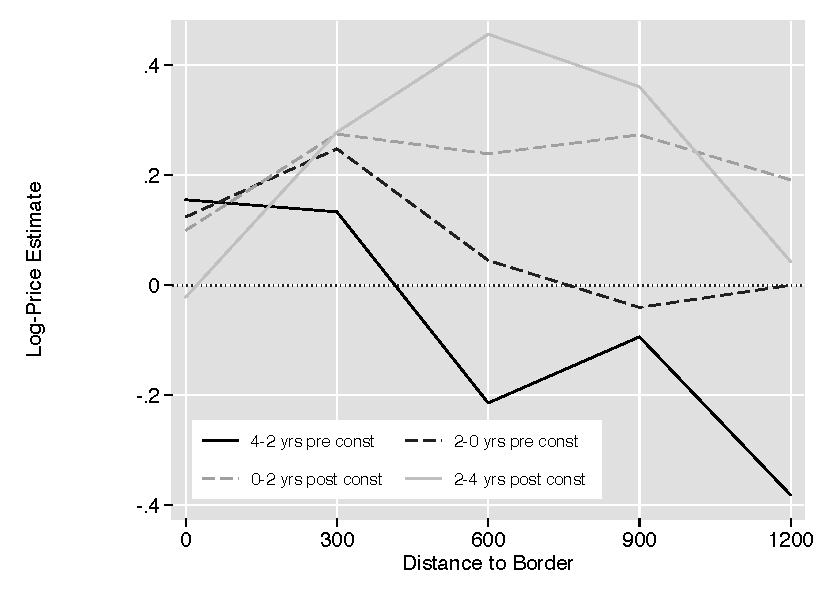
\includegraphics{figures/price_to_event_30.pdf}
% \end{figure}


\end{document}


